\documentclass[conference]{IEEEtran}
\IEEEoverridecommandlockouts
\renewcommand\IEEEkeywordsname{Keywords}
\usepackage[utf8]{inputenc}
\usepackage[T1]{fontenc}
\usepackage[american]{babel}
\usepackage[center]{caption}
\usepackage{graphicx}
\usepackage{svg}
\usepackage{listings}
\usepackage{float}
\usepackage{amsmath,amssymb,exscale}
\usepackage{blindtext, graphicx}
\usepackage{verbatim}
\usepackage{algorithm}
\usepackage{algpseudocode}
\usepackage{fancyvrb}
\usepackage{bera}
\usepackage{amsmath}
\usepackage{mathtools}
\usepackage{lipsum}
\usepackage{bm}

\usepackage{scalerel}
\usepackage{tikz}
\usetikzlibrary{svg.path}

\definecolor{orcidlogocol}{HTML}{A6CE39}
\tikzset{
  orcidlogo/.pic={
    \fill[orcidlogocol] svg{M256,128c0,70.7-57.3,128-128,128C57.3,256,0,198.7,0,128C0,57.3,57.3,0,128,0C198.7,0,256,57.3,256,128z};
    \fill[white] svg{M86.3,186.2H70.9V79.1h15.4v48.4V186.2z}
                 svg{M108.9,79.1h41.6c39.6,0,57,28.3,57,53.6c0,27.5-21.5,53.6-56.8,53.6h-41.8V79.1z M124.3,172.4h24.5c34.9,0,42.9-26.5,42.9-39.7c0-21.5-13.7-39.7-43.7-39.7h-23.7V172.4z}
                 svg{M88.7,56.8c0,5.5-4.5,10.1-10.1,10.1c-5.6,0-10.1-4.6-10.1-10.1c0-5.6,4.5-10.1,10.1-10.1C84.2,46.7,88.7,51.3,88.7,56.8z};
  }
}

\newcommand\orcid[1]{\href{https://orcid.org/#1}{\mbox{\scalerel*{

\begin{tikzpicture}[yscale=-1,transform shape]
\pic{orcidlogo};
\end{tikzpicture}
}{|}}}}

\usepackage[bookmarks=false]{hyperref}

\def\BibTeX{{\rm B\kern-.05em{\sc i\kern-.025em b}\kern-.08em
    T\kern-.1667em\lower.7ex\hbox{E}\kern-.125emX}}

\makeatletter 
\let\old@ps@headings\ps@headings 
\let\old@ps@IEEEtitlepagestyle\ps@IEEEtitlepagestyle 
\def\confheader#1{% 
\def\ps@headings{% 
\old@ps@headings% 
\def\@oddhead{\strut\hfill#1\hfill\strut}% 
\def\@evenhead{\strut\hfill#1\hfill\strut}% 
}% 
\def\ps@IEEEtitlepagestyle{% 
\old@ps@IEEEtitlepagestyle% 
\def\@oddhead{\strut\hfill#1\hfill\strut}% 
\def\@evenhead{\strut\hfill#1\hfill\strut}% 
}% 
\ps@headings% 
} 
\makeatother 

\confheader{% 
11th Workshop on Communication Networks and Power Systems (WCNPS 2026) 
} 

\begin{document}

\title{Evaluation of Indices for Monitoring the Voltage Stability Margin of Power Systems}

\author{\IEEEauthorblockN{Gonçalo Fontenele \orcid{0009-0008-1378-1420}\IEEEauthorrefmark{1}, Leonardo Rafael Bergonci Campos\IEEEauthorrefmark{1},
Murilo E. C. Bento\IEEEauthorrefmark{1}}
\IEEEauthorblockA{\IEEEauthorrefmark{1}Department of Electrical Engineering, Federal University of Rio de Janeiro\\
Rio de Janeiro, RJ 21941-909, Brazil\\
Email: goncalogfb@poli.ufrj.br, bergoncileo@gmail.com, murilobento@poli.ufrj.br}
}

\IEEEoverridecommandlockouts 
\IEEEpubid{\makebox[\columnwidth]{Copyright Notice } 
\hspace{\columnsep}\makebox[\columnwidth]{ }} 

\maketitle

\begin{abstract}
Voltage stability is a fundamental requirement for the secure operation of power systems, especially in operational scenarios close to transmission limits. This paper presents the development of a Python-based computational tool utilizing the Pandapower library for static voltage stability margin analysis. A Continuation Power Flow (CPF) algorithm featuring an adaptive step size strategy and distributed slack generation dispatch was implemented, designed to accurately replicate the solution methodology of the ANAREDE commercial software. The study validates the tool through a rigorous cross-comparison with ANAREDE using the IEEE 30-bus system, demonstrating negligible deviations. Furthermore, the tool's flexibility and adaptability are demonstrated on the IEEE 39-bus New England system. Additionally, a detailed comparative analysis of multiple Voltage Stability Indices (VSIs), such as FVSI, {mn}$, NLSI, NVSI, and the L-index, is performed, showcasing the correlation between these indicators and the imminence of voltage collapse.
\end{abstract}

\begin{IEEEkeywords}
Power Systems, Power System Stability, Voltage Stability, Continuation Power Flow, Stability Indices, Pandapower, ANAREDE.
\end{IEEEkeywords}

\section{Introduction}
\label{sec:introduction}
The evolution of power systems has increasingly posed significant challenges to operation centers worldwide \cite{Bhusal2020}. Growing uncertainty in hourly demand, the large-scale integration of intermittent renewable energy sources, the increasing occurrence of equipment failures and extreme weather conditions, and the vulnerability of communication infrastructures to cyberattacks all add substantial complexity to the continuous and secure operation of modern power systems. These emerging challenges underscore the need for new and effective tools to support operation centers in maintaining system reliability, resilience, and operational security.

Power system stability studies have become an essential task to ensure the safe and proper functioning of modern power systems \cite{Hatziargyriou2021}. Voltage stability assessment has gained prominence due to the increasingly stressed operation of power systems, driven by rising demand and the integration of renewable energy sources far from load centers \cite{Sun2019}. Voltage collapse, characterized by a progressive and uncontrollable drop in voltage levels across a significant portion of the system, is frequently associated with the inability of the transmission network and generators to meet the reactive power requirements of the load \cite{kundur1994power}.

To determine the security margin up to the point of collapse (known as the `nose'' of the PV curve), the industry widely employs the Continuation Power Flow (CPF) \cite{Ajjarapu1992}. Determining the point of maximum power transfer allows us to formulate the Voltage Stability Margin (VSM), which is the difference between the power levels in the nominal case and the case of maximum power transfer. Commercial software, such as ANAREDE (developed by CEPEL) in Brazil \cite{cepel2009anarede}, uses robust methods to bypass the singularity of the Jacobian matrix at the maximum transfer point. Reproducing these methods in an open academic environment is essential for developing new analytical metrics and control algorithms. 

The growth and evolution of information technologies, sensors, and communication have led to the development of smart grids \cite{Li2010}. Phasor Measurement Units (PMUs) ensure greater real-time observability of power systems. PMU data have shown promise in various voltage stability analysis and control applications, such as secondary voltage control. A relevant set of voltage stability indices have been developed to assess the proximity of the operating point to an instability mechanism such as voltage collapse \cite{modarresi2016comprehensive}.

This work proposes the development of a CPF simulator in Python, implementing step-size refinement and distributed generation dispatch techniques. The tool is rigorously validated by reproducing reference results on the IEEE 30-bus system. Building upon this baseline, a comparative study is introduced using the larger, heavily meshed IEEE 39-bus New England system. This dual-system approach enables a critical comparative analysis of several Voltage Stability Indices (VSIs) reviewed by \cite{modarresi2016comprehensive}, illustrating how network topology affects the predictive capability of these metrics.

\section{Theoretical Background}
\label{sec:background}

\subsection{Voltage Stability and PV Curve}
Voltage stability is the ability of a power system to maintain steady voltages at all buses after being subjected to a disturbance \cite{kundur1994power}. Collapse occurs when the system operates beyond the Maximum Power Transfer point, where the load impedance equals the Thevenin equivalent impedance of the network \cite{cutsem2007voltage}.

A classic approach to visualizing the voltage collapse phenomenon is through the PV curve, which relates the active power demanded at a load bus to the corresponding voltage level. As the loading increases, the voltage tends to decrease gradually until it reaches a critical point where small additional load variations produce abrupt changes in voltage. This point, known as the Maximum Loading Point (MLP), represents the static limit of the system and coincides with the saddle-node bifurcation.

\begin{figure}[htbp]
    \centering
    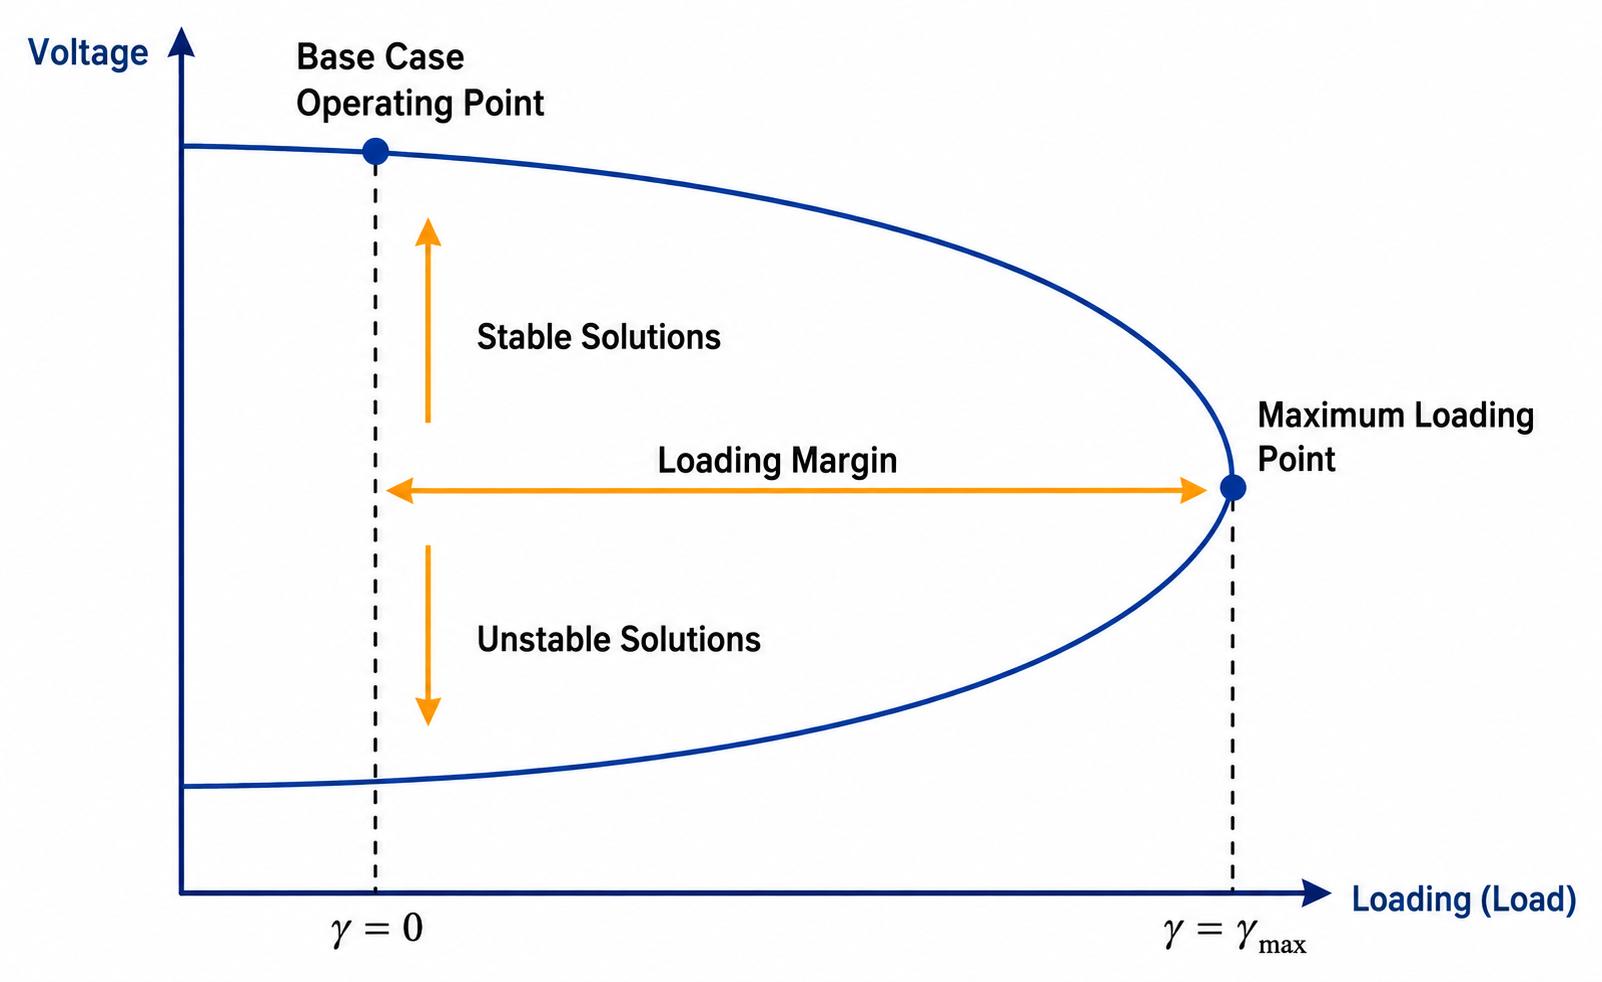
\includegraphics[width=\linewidth]{figures/curva_pv.png}
    \caption{Typical configuration of a PV curve, illustrating the voltage collapse phenomenon at the Maximum Loading Point (nose point).}
    \label{fig:curva_pv}
\end{figure}

\subsection{Review of Voltage Stability Indices (VSIs)}
Voltage Stability Indices (VSIs) are scalar metrics used to quantify the degree of proximity of an electrical system to voltage collapse. Based on the comprehensive review presented by Modarresi et al.~\cite{modarresi2016comprehensive}, six indicators used in the literature are analyzed: the line indices FVSI, {mn}$, NLSI, NVSI, and the nodal L-index.

The FVSI is derived from the quadratic form of the power flow equations for a radial line \cite{musirin2002}. Values close to 1 indicate that the reactive component of the load at the receiving bus is imposing significant stress on the line.
\begin{equation}
FVSI_{ij} = \frac{4 Z_{ij}^2 Q_j}{V_i^2 X_{ij}} \le 1.0
\end{equation}

The {mn}$ index evaluates the role of phase angle displacement and series impedance on stability \cite{moghavvemi98}:
\begin{equation}
L_{mn} = \frac{4 X_{ij} Q_j}{(V_i \sin(\theta - \delta))^2} \le 1.0
\end{equation}

Proposed to consider the influence of both active and reactive power on collapse, the NLSI expresses the weighted sum of $ and $ \cite{YazdanpanahGoharrizi2007}:
\begin{equation}
NLSI_{ij} = \frac{R_{ij} P_j + X_{ij} Q_j}{0.25 V_i^2} \le 1.0
\end{equation}

The NVSI uses the apparent power of the load, simultaneously capturing the effects of $ and $ \cite{kanimozhi2013novel}:
\begin{equation}
NVSI_{ij} = \frac{2 X_{ij} S_j}{2 Q_j X_{ij} - V_i^2} \le 1.0
\end{equation}

The L-Index utilizes the hybrid admittance matrix $. It measures the distance to collapse for each load bus $ \cite{kessel}:
\begin{equation}
L_j = \left| 1 - \sum_{i \in G} F_{ji} \frac{V_i}{V_j} \right|
\end{equation}

\section{Tool Development and Validation}
\label{sec:tool}

A flexible tool was developed in Python to simulate any network modeled in the Pandapower format. Before initiating the stability simulations, a comparative power flow test (Base Case) was performed between the developed tool and the ANAREDE software, utilizing the IEEE 30-bus system. The results demonstrated that the discrepancies found were statistically negligible (maximum voltage error $< 0.01\%$).

\subsection{Implemented Algorithm}
This work chose to replicate ANAREDE\'s logic instead of the tangent vector method. The implemented algorithm uses a Load Increment with Step Refinement approach. The initial state of the network is set based on the power flow results of the base case. A load increment ($\lambda$) is applied to the load buses, and simultaneously, the generator dispatch is adjusted (Distributed Slack). If the Newton-Raphson solver fails to converge, the algorithm discards the current iteration, restores the network state, and cuts the increment step in half. This repeats until a minimum precision (^{-4}$ p.u.) is reached. To optimize computational performance, sparse linear algebra was utilized for calculating indices like the L-Index.


\begin{figure}[htbp]
    \centering
    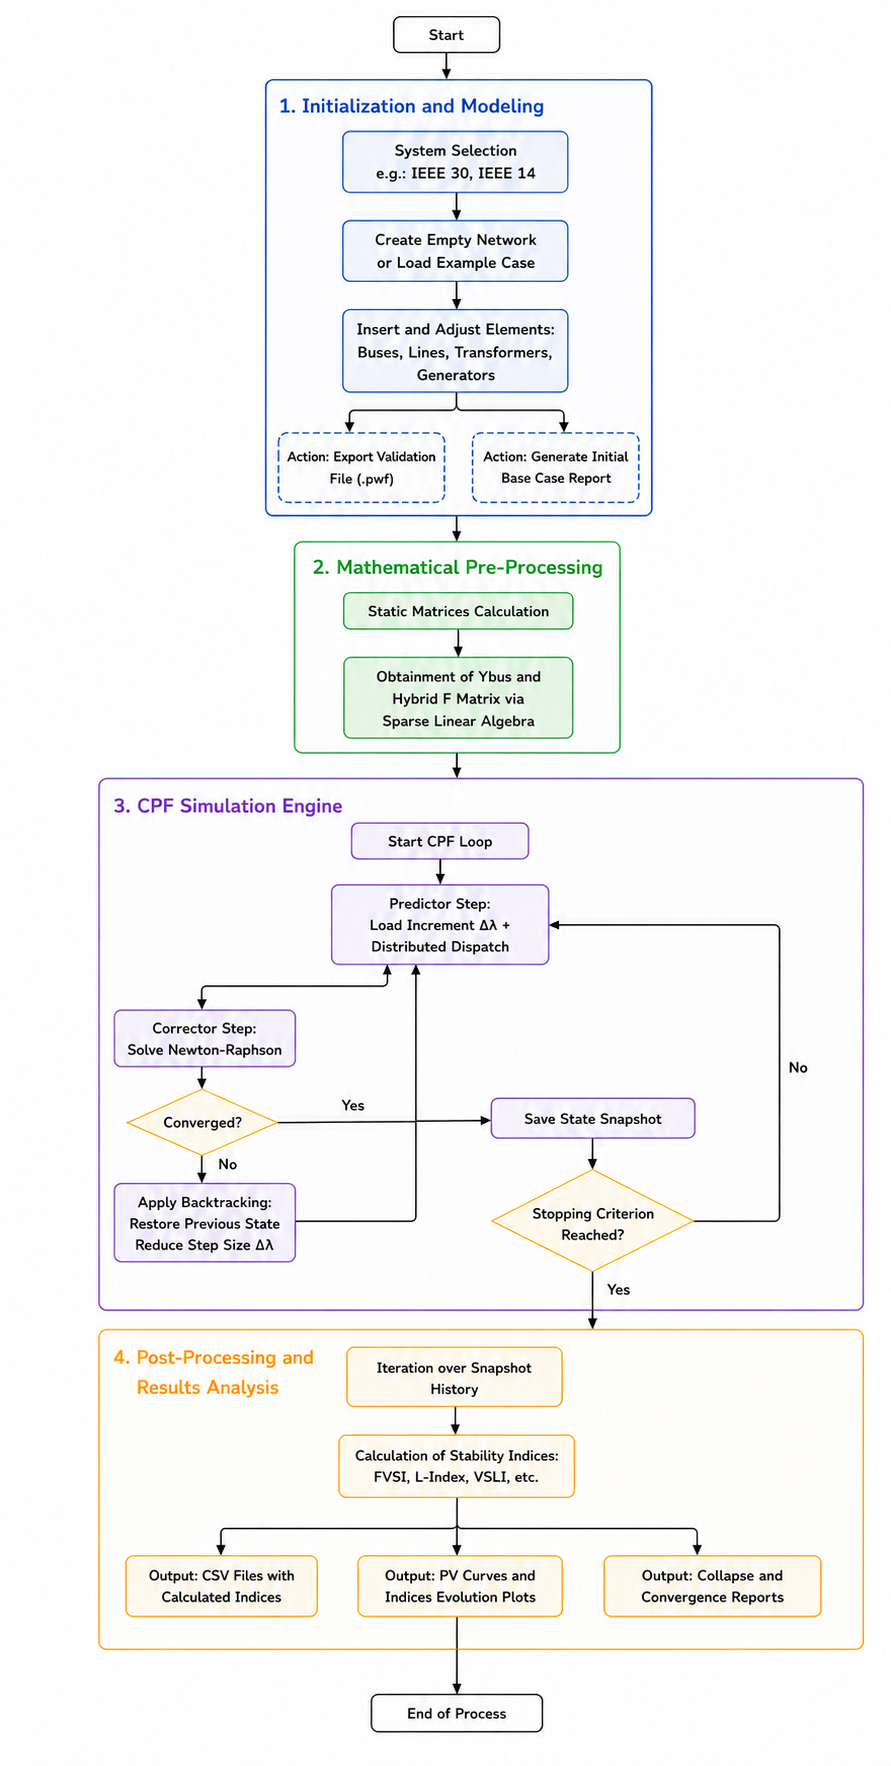
\includegraphics[width=\linewidth]{figures/fluxograma.png}
    \caption{Flowchart detailing the computational architecture and execution steps of the Continuation Power Flow algorithm.}
    \label{fig:fluxograma}
\end{figure}

\section{Results and Discussion}
\label{sec:results}

\subsection{Stability Margin (IEEE 30-Bus)}
The simulation on the IEEE 30-bus ANAREDE Equivalent system was configured with reactive generation limits relaxed and simultaneous increment of P and Q. The process reached the point of collapse with a total loading of 808.58 MW ($\lambda \approx 2.853$). This value represents the true physical margin without the influence of automated transformer taps. The adaptive step size algorithm allowed for a smooth tracking of the curve, reducing the step automatically as it approached the singularity.

\begin{figure}[htbp]
    \centering
    \includesvg[width=\linewidth]{figures/fig_pv_30.svg}
    \caption{PV curves of the IEEE 30-bus system simulated via the developed Python tool, highlighting the critical collapse threshold at 808.58 MW.}
    \label{fig:curvapv}
\end{figure}

\subsection{VSI Statistical Correlation Analysis}
To understand how different indices respond to the stress imposed by load increments near the collapse point, a Spearman rank correlation analysis was performed between the evaluated VSIs at the final iteration (MLP) of the IEEE 30-bus system. The Spearman coefficient ($\rho$) measures the monotonic relationship between two variables.

\begin{table}[htbp]
\centering
\caption{Spearman Rank Correlation between VSIs at Collapse Point}
\label{tab:spearman}
\begin{tabular}{lccccc}
\toprule
Index & FVSI & {mn}$ & NLSI & NVSI & L-Index \\ \midrule
FVSI & 1.0000 & 0.9963 & 0.8545 & 0.7115 & -0.1869 \\
{mn}$ & 0.9963 & 1.0000 & 0.8822 & 0.7451 & -0.1733 \\
NLSI & 0.8545 & 0.8822 & 1.0000 & 0.8535 & -0.0391 \\
NVSI & 0.7115 & 0.7451 & 0.8535 & 1.0000 & -0.0613 \\
L-Index & -0.1869 & -0.1733 & -0.0391 & -0.0613 & 1.0000 \\ \bottomrule
\end{tabular}
\end{table}

Table \ref{tab:spearman} reveals a very high correlation between FVSI and {mn}$ ($\rho = 0.9963$), indicating that they capture nearly identical stress rankings across transmission lines. NLSI and NVSI also present a strong correlation between themselves and with FVSI, as all are line-based indices structurally dependent on line impedance parameters. In contrast, the L-Index, being a nodal index dependent on the global admittance matrix, exhibits near-zero or slightly negative correlation with the line indices. This proves that nodal indices and line indices evaluate completely orthogonal aspects of voltage stability, reinforcing the necessity of using both categories in conjunction.

\subsection{Influence of Network Topology (IEEE 39-bus)}
To broaden the scope of the study, the highly meshed IEEE 39-bus New England system was utilized. The behavior of line indices in robust and meshed grids differs significantly from radial or weaker systems. As the system was driven to collapse, it was observed that rather than a few lines peaking abruptly, multiple interconnected components experienced a simultaneous, gradual rise in their index values.

This distributed stress phenomenon occurs because the meshed topology naturally offers parallel paths for power flow. Consequently, when a specific corridor becomes saturated, the power is redirected through alternative lines, balancing the stress. As a result, line indices may be less effective at pinpointing a single point of failure in heavily meshed grids, as illustrated by the NLSI index evolution in Fig. \ref{fig:nlsi_39}.

\begin{figure}[htbp]
    \centering
    \includesvg[width=\linewidth]{figures/analise_nlsi_39.svg}
    \caption{Response of the NLSI line index to loading increments, highlighting shared transmission burdens across the IEEE 39-bus grid.}
    \label{fig:nlsi_39}
\end{figure}

In contrast, the nodal L-Index successfully highlighted the most vulnerable load buses in the 39-bus system as it approached the MLP (Fig. \ref{fig:lindex_39}), demonstrating its analytical robustness and independence from the grid\'s meshing characteristics.

\begin{figure}[htbp]
    \centering
    \includesvg[width=\linewidth]{figures/analise_l_index_39.svg}
    \caption{Nodal vulnerability mapping using the L-Index in the complex IEEE 39-bus topology, maintaining predictive accuracy regardless of grid meshing.}
    \label{fig:lindex_39}
\end{figure}


\begin{figure}[htbp]
    \centering
    \includesvg[width=\linewidth]{figures/fig_pv_39.svg}
    \caption{PV curves of the IEEE 39-bus New England system, demonstrating behavior in heavily meshed grids.}
    \label{fig:pv_39}
\end{figure}

\section{Conclusions}
\label{sec:conclusions}
This work presented a Python-based computational tool for voltage stability assessment, accurately reproducing commercial software methodologies like adaptive step refinement. The validation on the IEEE 30-bus system confirmed the robustness of the implementation and allowed determination of the baseline physical limit of 808 MW for the static PV curve analysis without automated tap interference.

The statistical and comparative analysis of stability indices highlighted that line indices (like FVSI and {mn}$) are highly correlated among themselves but orthogonal to nodal indices (L-Index). Furthermore, the application to the meshed IEEE 39-bus system demonstrated that line indices tend to show distributed stress in redundant topologies, while the L-Index maintains its predictive accuracy. The combined use of both metric classes provides a comprehensive view for monitoring operational safety margins.

\bibliographystyle{IEEEtran}
\bibliography{refs}

\end{document}
